
\subsection{Iterativ}

Das Modell wird auch \textbf{Sprialmodell}\footnote{
    s.a. \url{https://de.wikipedia.org/wiki/Spiralmodell}, abgerufen 27.03.2024
} genannt und geht auf \textit{Boehm} zurück (vgl.~\cite[]{Boe88}).\\

\noindent
Die Entwicklung wird in \textbf{zeitliche Iterationen} gleicher Länge unterteilt\footnote{
    i.d.R. dauern diese zwischen $2$ und $6$ Wochen
}.\\
Innerhalb einer Iteration wird ähnlich wie beim Wasserfallmodell vorgegangen\footnote{
\textit{Balzert} betont, dass das Spiralmodell ein \textbf{evolutionäres} Vorgehensmodell ist und innerhalb der Phasen das geeigneste Prozessmodell ausgewählt werden kann (vgl.\cite[556]{Bal08})
}.\\
Das Ergebnis einer Iteration kann in der nächsten Iteration weiterbearbeitet und verbessert werden\footnote{
    eine Iteration wird normalwerweise kein fertiges Teilsystem zur Abnahme liefern, aufgrund der kurzen Dauer
}.\\
In einer Iteration werden zunächst die risikoreichsten Aufgaben bearbeitet, um das Risiko im Verlauf des Projektes zu minimieren.\\

\noindent
Bei der Anwendung dieser Vorgehensweise ist es nicht zwingend notwendig, in jeder Iteration alle Phasen  durchzuexerzieren, bspw. wenn ein Prototyp entwickelt wird, der in dieser Phase nicht vollständig getestet werden muss.\\
Gleichzeitig zeichnet sich die Endphase eines iterativ durchgeführten Projektes dadurch aus, dass die letzten Iterationen nur noch für Tests verwendet werden (vgl. Abbildung~\ref{fig:iterativ}).

\begin{figure}
    \centering
    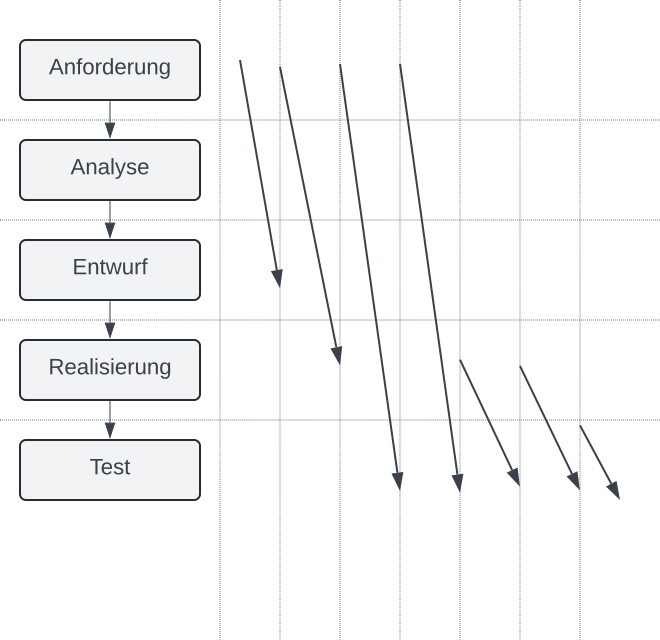
\includegraphics[scale=0.4]{chapters/Prozessmodelle/img/iterativ}
    \caption{Bei der Anwendung des iterativen Modells können einzelne Phasen überprungen werden. (Quelle: in Anlehnung an \cite[28, Abb. 3.3]{Wed09})}
    \label{fig:iterativ}
\end{figure}

\subsubsection*{RUP}
Die bekannteste iterative Vorgehensweise ist der \textbf{Rational Unified Process} (\textit{RUP})\footnote{
    s. \url{https://en.wikipedia.org/wiki/Rational_unified_process}, abgerufen 27.03.2024
}.\\
Angelehnt an das Wasserfallmodell werden bei \textit{RUP} Iterationen aufgeteilt in

\begin{enumerate}
    \item \textit{Inception} (Vorbereitung)
    \item \textit{Elaboration} (Ausarbeitung d. Architektur)
    \item \textit{Construction} (Konstruktion)
    \item \textit{Transition} (Auslieferung)
\end{enumerate}

\noindent
Wie im Wasserfallmodell werden hier für die einzelnen Phasen Ergebnis-Artefakte geliefert, wie Anwendungsfälle oder Klassendiagramme.


\subsubsection*{Vorteile}

\begin{itemize}
    \item Kunde kann bereits am Ende einer Iteration Ergebnisse sehen und dadurch Einfluss auf die nächste Iteration nehmen.
    \item Neue Anforderungen können in einer folgenden Iteration aufgenommen werden.
    \item Implementierung flexibler, da Entwickler durch die \textit{lessons-learned} Erfahrungen kurzfristig in eine nächste Iteration einfliessen lassen können.
\end{itemize}

\noindent
\textit{Balzert} stellt fest, dass das Spiralmodell ein \textbf{evolutionäres Modell} in der Hinsicht ist, als dass es ``entsprechend der jeweiligen Entwicklungssituation das nächste zu verwendende Prozessmodell auswählt.`` (\cite[556]{Bal08}).

\subsubsection*{Nachteile}

\begin{itemize}
    \item Das Ergebnis der Entwicklung ist vorher nicht festgelegt, die Anforderungen entstehen erst im Laufe der Iterationen.
    \item[] $\rightarrow$ hierdurch können Probleme bei der Projektplanung / Budgetierung entstehen, da die Kosten-Nutzen-Analyse für den Auftraggeber und die die Aufwandsabschätzung für den Auftragnehmer schwer fällt, was die Vertragsgestaltung komplizierter macht.
\end{itemize}

\subsubsection*{Iterativ-Inkrementelles Vorgehen}
Bei länger laufenden Projekten sollte man prüfen, ob die Entwicklung nicht zusätzlich in Inkremente gegliedert werden kann, um die Anforderungen und erwarteten Ergebnisse besser abstecken zu können.

